\documentclass[8pt,a4paper,landscape]{extarticle}

\usepackage[utf8]{inputenc}
\usepackage[T1]{fontenc}
\usepackage[ngerman]{babel}
\usepackage[page]{totalcount}

\usepackage{geometry}
\usepackage{titlesec}
\usepackage{fancyhdr}

\usepackage{amsmath}
\usepackage{amssymb}

\usepackage{listings}
\usepackage{enumitem}

\usepackage{graphicx}
\usepackage{tabularx}

\usepackage{multicol}

\hyphenation{
}

% define some static variables %
\def\creator{Louis Seubert}
\def\subject{Interaktivesysteme}
\def\maxpage{5}

% rotate page and set margins %
\geometry{left=0.55cm,right=0.55cm,top=1.10cm,bottom=0.55cm,landscape,headsep=2mm}

% make header and footer %
\pagestyle{fancy}
\fancyhead{} % clear header
\fancyhead[L]{Zusammenfassung \subject}
\fancyhead[R]{\thepage\;von\;\maxpage}
\fancyhead[C]{\creator}
\fancyfoot{} % clear footer

% configure document %
\setitemize{leftmargin=15pt}
\setenumerate{leftmargin=15pt}
\setlist{itemsep=1pt,parsep=1pt}

\setlength{\parindent}{0pt}
\setlength{\parskip}{0pt}
\setlength{\topskip}{10pt}
\setlength{\columnseprule}{0.5pt} % column seperator line

% change style %
\titleformat*{\section}{\large\bfseries}
\titlespacing*{\section}{0pt}{4pt}{0pt}

\titleformat*{\subsection}{\normalsize\bfseries}
\titlespacing*{\subsection}{0pt}{4pt}{0pt}

\titleformat*{\subsubsection}{\normalsize\bfseries}
\titlespacing*{\subsubsection}{0pt}{4pt}{0pt}

\titleformat*{\paragraph}{\normalsize\bfseries}
\titlespacing{\paragraph}{0pt}{.5em}{.5em}

\titleformat*{\subparagraph}{\small\bfseries}
\titlespacing*{\subparagraph}{0pt}{.5em}{.5em}

\title{Zusammenfassung \subject} 
\author{\creator}

% define some macros %
\newcommand{\example}{\textit{\underline{Beispiel:} }}

% define some enviroments %

\newenvironment{definitions}{
	\par\vspace{\abovedisplayshortskip}\noindent
	\tabularx{\columnwidth}{>{$}l<{$} @{${}={}$} >{\raggedright\arraybackslash}X}
}{\endtabularx\par\vspace{\belowdisplayshortskip}}

\begin{document}
\begin{multicols*}{4}
	\section{Einführung}
	\subsection{Unterscheidung Anwender \(\leftrightarrow\) Benutzer}
	\begin{description}
		\item[Anwender] sind Entitäten, welche direkt oder auch indirekt ein
		      Hilfsmittel zur Erzielung eines Vorteils verwendeen
		\item[Benutzer] sind natürliche Personen, die direkt mit einem
		      Hilfsmittel arbeiten, um einen Vorteil zu erzielen
	\end{description}
	\example Ein Direktor (Anwender) lässt sich von seinem Chauffeur (Benutzer)
	mit einem Auto (Hilfsmittel) zu seinem nächsten Termin bringen
	\subsection{Definition Interaktives System}
	Ein \textbf{interaktives System} gibt dem Benutzer die Möglichkeit, mittels
	einer Benutzerschnittstelle die laufende Bearbeitung einer Aufgabe durch ein
	technisches System zu beeinflussen.
	\subsection{Formen von Interaktion}
	\begin{itemize}[itemsep=1pt, parsep=1pt, nolistsep]
		\item \textbf{Anweisung}
		      \begin{itemize}[itemsep=1pt, nolistsep]
			      \item Eingabe von Kommandos
		      \end{itemize}
		\item \textbf{Dialog}
		      \begin{itemize}[itemsep=1pt, nolistsep]
			      \item Ablauf von Eingabe und Ausgabe
		      \end{itemize}
		\item \textbf{Manipulation (von Kommandos, Inhalten)}
		      \begin{itemize}[itemsep=1pt, parsep=1pt, nolistsep]
			      \item Auswählen („Choice“)
			      \item Ansteuern („Target Acquisition“)
			      \item Verändern
		      \end{itemize}
		\item \textbf{Erkunden (einer Menge von Kommandos, Inhalten)}
		      \begin{itemize}[itemsep=1pt, parsep=1pt, nolistsep]
			      \item Suchanfragen
			      \item Browsing
		      \end{itemize}
	\end{itemize}
	\subsection{Arten von Benutzerschnittstellen}
	\begin{itemize}
		\item \textbf{T}ext \textbf{U}ser \textbf{I}nterface
		\item \textbf{T}angible \textbf{U}ser \textbf{I}nterface
		\item \textbf{G}raphical \textbf{U}ser \textbf{I}nterface
		\item \textbf{V}oice \textbf{U}ser \textbf{I}nterface
		\item \textbf{H}aptic \textbf{U}ser \textbf{I}nterface
		\item \textbf{N}atural \textbf{U}ser \textbf{I}nterface\par
		      (möglichst wenig zu erlernende Eingabegeräte)
		\item \textbf{I}ntuitive \textbf{U}ser \textbf{I}nterface\par
		      (möglichst leicht erlernbare Eingabegeräte)
		\item \textbf{B}rain \textbf{C}omputer \textbf{I}nterface
		\item \textbf{C}ommand \textbf{L}ine \textbf{I}nterpreter
	\end{itemize}
	\subsection{Fallstudien}
	\subsubsection*{Sketchpad}
	Programm entwickelt von Ivan Sutherland im Rahmen einer Doktorarbeit. \\
	Mittels Lichtgriffel: Zeichnen und Deformieren geometrischer Objekte;
	Vektorgraphiken; Erste objektorientierte Ansätze zur Bedienung
	\subsubsection*{Xerox Alto}
	Kommandozeileninterpreter Alto Executive: Graphische Oberfläche;
	Mehrere Applikationen; Mehrere Fenster
	\subsubsection*{Apple Macintosh}
	Features u.a. Desktop-Metapher, Drop-Down-Menüs, Ordner, Mülleimer sowie
	überlappende Fenster
	\subsubsection*{Windows 1.0}
	Zeigegerät, Menüs, Statuszeile, Symbole, Zwischenablage, Taskleiste.
	Wegen Vektorgrafik-Fähigkeit bereits als GUI (und nicht als TUI)
	klassifiziert.
	\section{Zeigegeräte}
	\subsection{Einteilung von Interaktionstechnologien}
	Nach \emph{Krauß}
	\begin{itemize}[nolistsep]
		\item Koordinatengebend
		      \begin{itemize}[nolistsep]
			      \item Dimensionalität
			            \begin{itemize}[nolistsep]
				            \item[\(\rightarrow\)] eindimensional,
				                  zweidimensional, mehrdimensional
			            \end{itemize}
			      \item Verhältnis Lage zu Wirkort
			            \begin{itemize}[nolistsep]
				            \item[\(\rightarrow\)] Indirekt wirkende vs. direkt
				                  wirkende
			            \end{itemize}
		      \end{itemize}
		\item Nicht koordinatengebend
		      \begin{itemize}[nolistsep]
			      \item Tasten
			      \item Sprache
			      \item Gesten
		      \end{itemize}
	\end{itemize}
	\subsection{Koordinatengebende}
	\subsubsection{Direkte Zeigegeräte}
	\begin{itemize}
		\item Es wird unmittelbar auf die Ausgabe gezeigt
		\item Merkmale
		      \begin{itemize}[nolistsep]
			      \item Lernaufwand Bedienung Zeigegeräts minimal
			      \item Verdeckung der Ausgabe durch Zeigegerät
			      \item Ermüdungserscheinungen
		      \end{itemize}
		\item \example Touchscreen
	\end{itemize}
	\subsubsection{Indirekte Zeigegeräte}
	\begin{itemize}
		\item Nicht im direkten Kontakt mit der Ausgabe
		\item Bewegung an anderer Stelle und Transformation der Koordinaten an
		      den Bildschirm
		\item Merkmale
		      \begin{itemize}[nolistsep]
			      \item Lernaufwand Bedienung des Zeigegeräts \\
			            z.B. Hand-Augen-Koordination bei Computermaus
			      \item Kopplung zwischen Zeigegerät und Ausgabe als
			            modulierbarer Parameter
		      \end{itemize}
		\item \example Computermaus
	\end{itemize}
	\subsubsection{Positionierung}
	\paragraph{Absolute Positionierung} Eindeutige Zuordnung der Position des
	Zeigegerätes zur Position auf dem Bildschirm. Der Bezug zum Ursprung kann
	gegeben sein.
	\paragraph{Relative Positionierung} Es wird von aktuell gespeicherter
	Position ausgegangen und die Veränderung der Koordinaten umgesetzt.
	\paragraph{Control-Display-Gain} \textbf{<<MacKenzie>>} Der durch die
	Bewegung eines indirekten Zeigegerätes („Control“) resultierende Effekt
	(„Gain“) am Bildschirm. \\
	Nach MacKenzie balanciert eine günstige Einstellung des Gain Schnelligkeit
	und Präzision der Positionierung.
	\begin{center}
		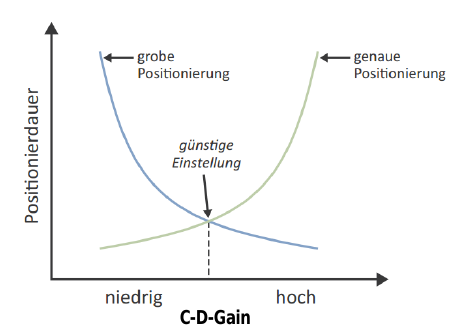
\includegraphics[width=0.7\linewidth]{./pictures/figure_01.png}
	\end{center}
	\begin{itemize}
		\item \textit{Gain niedrig:} Große Bewegung Controller bewirkt
		      durchschnittlichen Effekt; Vorteilhaft für Feinpositionierung
		\item \textit{Gain hoch:} Kleine Bewegung Controller bewirkt
		      durchschnittlichen Effekt; Vorteilhaft für Grobpositionierung
	\end{itemize}
	\subsubsection{Physikalische Charakterisierung}
	\paragraph{Abtastrate}
	\begin{itemize}
		\item Erfassung der Position und Tasten des Zeigegerätes zu diskreten
		      Zeitabständen
		\item Definiert die zur Positionsbestimmung verfügbare Zeit
	\end{itemize}
	\begin{center}
		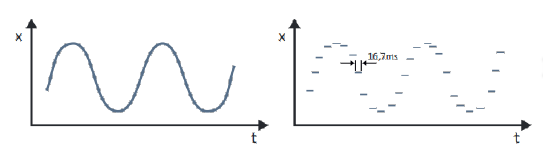
\includegraphics[width=\linewidth]{./pictures/figure_02.png}
	\end{center}
	\paragraph{Verzögerung}
	\begin{itemize}
		\item Zeitabstand zwischen Abtastung und Änderung am Bildschirm
		\item Verzögerung sollte geringer als die Hälfte der Abtastrate sein
		\item Schon geringe Verzögerungen bringen höhere Fehlerrate bei
		      Selektionen mit sich
	\end{itemize}
	\paragraph{Genauigkeit}
	\begin{itemize}
		\item Genauigkeit: Abweichung der durch einen Sensor gemessenen Position
		      von der tatsächlichen Position
		\item Gemeinsame Optimierung von Genauigkeit und Abtastrate nicht
		      möglich
		      \begin{itemize}[nolistsep]
			      \item Obergrenze bildet die räumliche Auflösung des Sensors
			      \item Hohe Abtastrate geht zu Lasten der Genauigkeit
		      \end{itemize}
	\end{itemize}
	\paragraph{Abhängigkeit von der individuellen Anwendung}
	\begin{itemize}
		\item Bei Interaktion in komplexen virtuellen Welten in modernen
		      Computerspielen oder 3D-Modellierungstools können hohe
		      Anforderungen an Zeigegeräte gestellt werden
	\end{itemize}
	\subsubsection{Zeigeaufgaben}
	\begin{center}
		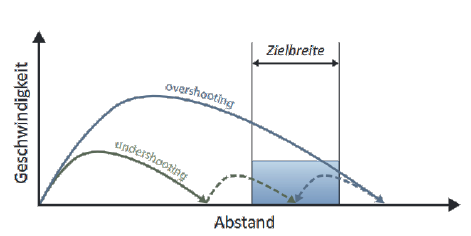
\includegraphics[width=0.7\linewidth]{./pictures/figure_03.png}
	\end{center}
	Das Experiment nach Fitts: Wie lange benötigt ein Mensch, um mit einm Stift
	ausgehend von einem Startpunkt ein Ziel zu erreichen? Das Experiment steht
	dabei in der Abhängigkeit von der Distanz \(D\) des Ziels und der Breite
	\(W\).
	\paragraph{Fitts}
	\[MT = a + b \cdot ID\]
	\[ID = \log_{2}\left(\frac{2D}{W}\right)\]
	\paragraph{MacKenzie}\mbox{}\\
	Verbesserung der Formel von Fitts
	\[ID = \log_{2}\left(\frac{D}{W} + 1\right)\]
	\paragraph{Accot \& Zhai}\mbox{}\\
	Berücksichtigt auch Höhe und y-Koordinate des Ziels
	\[MT = a + b \cdot \log_{2}\left(\sqrt{\left(\frac{D}{W}\right)^{2}+\eta\left(\frac{D}{H}\right)^{2}} + 1\right)\]
	\subsubsection{Ergebnisse des Praktikumsversuchs}
	MacKenzie > Accot/Zhai > Fitts
	\begin{itemize}
		\item In Fitts' Experiment wird ein direktes Zeigegerät benutzt
		\item \emph{Precuing} macht eine Zeigeaufgabe immer einfacher
		\item \emph{Reset} macht eine Zeigeaufgabe zunächst schwerer, jedoch
		      kann es schnell erlernt werd
	\end{itemize}
	\subsubsection{Unterstützung von Zeigeaufgaben}
	\paragraph{Anpassung Bedienelemente} Eine Anpassung der Größe, Anordnung,
	Form. \\ Verkleinern ist nach Fitts schwieriger und die Unterscheidbarkeit
	nimmt ab.
	\paragraph{Temporäre Modifikation des Interface} Eine Anpassung des User
	Interface. \\ Nach Parker kann man das Ziel oder den Cursor vergrößern,
	sowie den Cursor zum Ziel bewegen oder auch das Ziel zum Cursor bewegen. \\
	\underline{Nachteile:} Eine Veränderung des User Interface kann den Benutzer
	irritiren; Aussagen über eine Selektionsinteraktion sind schwer
	\paragraph{Mehrere Mauszeiger} \underline{Nachteile:} Potentiell mehrdeutige
	Zielauswahl
	\subsubsection{Direct Manipulation}
	Direkt manipulative Interfaces zeichnen sich aus nach \emph{Hutchins et al.}
	durch:
	\begin{itemize}
		\item Geringe Distanz
		      \begin{itemize}[nolistsep]
			      \item von Benutzerzielen
			      \item zu deren Erreichung nötigen Interaktionen
		      \end{itemize}
		\item Hohes Engagement
		      \begin{itemize}[nolistsep]
			      \item direkte Auseinandersetzung des Benutzers
			      \item mit dem Objekt von Interesse
		      \end{itemize}
		\item \example
		      \begin{itemize}[nolistsep]
			      \item Skript schreiben:\\ Distanz hoch, Engagement niedrig
			      \item Drag \& Drop:\\ Distanz niedrig, Engagement hoch
		      \end{itemize}
	\end{itemize}
	\paragraph{Prinzipien nach Shneiderman}
	\begin{itemize}
		\item Kontinuierliche Repräsentation des Objekts von Interesse
		\item Eingabe auf Basis einfacher physikalische Aktionen
		      (z.B. Bewegung der Maus) anstelle sprachbasierter Kommandos
		\item Schnelle, schrittweise, umkehrbare Operationen, deren Auswirkung
		      auf das Objekt von Interesse unmittelbar erkennbar wird
		\item Schrittweises Erlernen der Interaktion ausgehend von minimalem
		      Vorwissen
	\end{itemize}
	\paragraph{Vorteile nach Shneiderman}
	\begin{itemize}
		\item Anfänger können die grundlegende Funktionen schnell erlernen,
		      beispielsweise nach Vorführung durch einen erfahreneren Benutzer
		\item Interaktionskonzepte werden nach längerer Nichtanwendung leicht
		      erinnert
		\item Benutzer können unmittelbar erkennen, ob sie sich durch Aktionen
		      ihren Zielen annähern – und gegebenenfalls ihre Aktionen anders
		      ausrichten
		\item Benutzer sind weniger zögerlich im Umgang mit dem System, da
		      Aktionen leicht verständlich und umkehrbar sind
		\item Benutzer erleben Kontrolle über das System und können dessen
		      Reaktionen direkt beobachten
	\end{itemize}
\end{multicols*}
\end{document}
